\hypertarget{group__Build}{\section{Build}
\label{group__Build}\index{Build@{Build}}
}


Build tools for test content.  


Collaboration diagram for Build\-:
\nopagebreak
\begin{figure}[H]
\begin{center}
\leavevmode
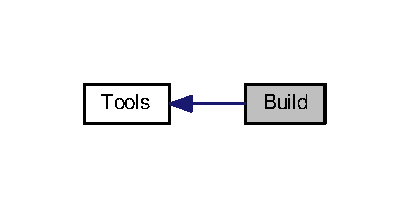
\includegraphics[width=196pt]{group__Build}
\end{center}
\end{figure}
Build tools for test content. \hypertarget{group__Build_Autotools}{}\subsection{Autotools}\label{group__Build_Autotools}
Run typical autotools commands to configure and build a software package 
\begin{DoxyParams}{Parameters}
{\em middleware} & Middleware stage that these tests are to be built against \\
\hline
{\em parent} & Section that precedes this one in the dependency tree \\
\hline
{\em autogen\-\_\-cmd} & Command to be executed to setup the configure script, usually called autogen.\-sh or autogen.\-pl \\
\hline
{\em configure\-\_\-options} & Options to be passed to configure. Note that the prefix will be automatically set and need not be provided here \\
\hline
{\em make\-\_\-options} & Options to be passed to the make command \\
\hline
{\em build\-\_\-in\-\_\-place} & Build tests in current location (no prefix or install) \\
\hline
{\em merge\-\_\-stdout\-\_\-stderr} & Merge stdout and stderr into one output stream \\
\hline
{\em stdout\-\_\-save\-\_\-lines} & Number of lines of stdout to save \\
\hline
{\em stderr\-\_\-save\-\_\-lines} & Number of lines of stderr to save \\
\hline
{\em modules} & Modules to load \\
\hline
{\em modules\-\_\-unload} & Modules to unload\\
\hline
\end{DoxyParams}
\hypertarget{group__Build_Hostfile}{}\subsection{Hostfile}\label{group__Build_Hostfile}
Builds a hostfile based on a nodelist 
\begin{DoxyParams}{Parameters}
{\em parent} & Section that precedes this one in the dependency tree \\
\hline
{\em nodelist} & list of nodes to create hostfile from \\
\hline
{\em hostfile} & name of hostfile to generate\\
\hline
\end{DoxyParams}
\hypertarget{group__Build_Shell}{}\subsection{Shell}\label{group__Build_Shell}
Run shell commands to configure and build a software package 
\begin{DoxyParams}{Parameters}
{\em middleware} & Middleware stage that these tests are to be built against \\
\hline
{\em command} & Command to execute \\
\hline
{\em parent} & Section that precedes this one in the dependency tree \\
\hline
{\em merge\-\_\-stdout\-\_\-stderr} & Merge stdout and stderr into one output stream \\
\hline
{\em stdout\-\_\-save\-\_\-lines} & Number of lines of stdout to save \\
\hline
{\em stderr\-\_\-save\-\_\-lines} & Number of lines of stderr to save \\
\hline
{\em modules} & Modules to load \\
\hline
{\em modules\-\_\-unload} & Modules to unload \\
\hline
{\em fail\-\_\-test} & Specifies whether this test is expected to fail (value=None means test is expected to succeed) \\
\hline
{\em fail\-\_\-returncode} & Specifies the expected failure returncode of this test \\
\hline
{\em allocate\-\_\-cmd} & Command to use for allocating nodes from the resource manager \\
\hline
{\em deallocate\-\_\-cmd} & Command to use for deallocating nodes from the resource manager \\
\hline
{\em asis\-\_\-target} & Specifies name of asis\-\_\-target being built. This is used with "A\-S\-I\-S" keyword to determine whether to do anything. \\
\hline
\end{DoxyParams}
